\documentclass[11pt]{article}
\usepackage[utf8]{inputenc}
\usepackage{amsmath}
\usepackage{amsfonts}
\usepackage{amssymb}
\usepackage{graphicx}
\usepackage[super]{nth}
\usepackage{amsthm}
\usepackage{bm}
\newtheorem{theorem}{Theorem}
\newtheorem{objective}{Objective}
\newtheorem{model}{Model}
\usepackage{xcolor}
\definecolor{light-gray}{gray}{0.95}
\newcommand{\code}[1]{\colorbox{light-gray}{\texttt{#1}}}
\usepackage{listings}
\usepackage{placeins}
\usepackage{enumitem}
\usepackage[T1]{fontenc}

\usepackage[authoryear]{natbib}

\lstset{language=R}


\makeatletter
\renewcommand{\maketitle}{
\begin{center}

\pagestyle{empty}

{\Large \bf \@title\par}
\vspace{1cm}

{\LARGE Marcel Gietzmann-Sanders}\\[1cm]

STAT651 - Statistical Theory I \\
University of Alaska Fairbanks


\end{center}
}\makeatother


\title{Exam 2 - Take-home}

\date{2025}
\setcounter{tocdepth}{2}
\begin{document}
\maketitle

\section*{Question 1}

I'm going to assume that $f_Y(y)=\frac{1}{b}f_X\left(\frac{x-a}{b}\right)$ was supposed to be $f_Y(y)=\frac{1}{b}f_X\left(\frac{y-a}{b}\right)$ as $\frac{1}{b}f_X\left(\frac{x-a}{b}\right)$ does not integrate to $1$ over the support of $X$ unless $a=0,b=1$ and therefore is not in fact a pdf. 

Under this assumption $Y$ is a location scale family of $X$ where $Y=a+bX$. As a location scale family the mean will be $\mathbb{E}(Y) = \mathbb{E}(X) + a$ and the variance $Var(Y) = b^2Var(X)$. Therefore as $\mathbb{E}(X)=Var(X)=1$ we need to set $a=-1,b=1$ to get:

$$f_Y(y)=e^{-(y+1)}I(y\geq -1)$$

\newpage

\section*{Question 2}

\subsection*{a)}

\begin{figure}[h!] 
	\centering
  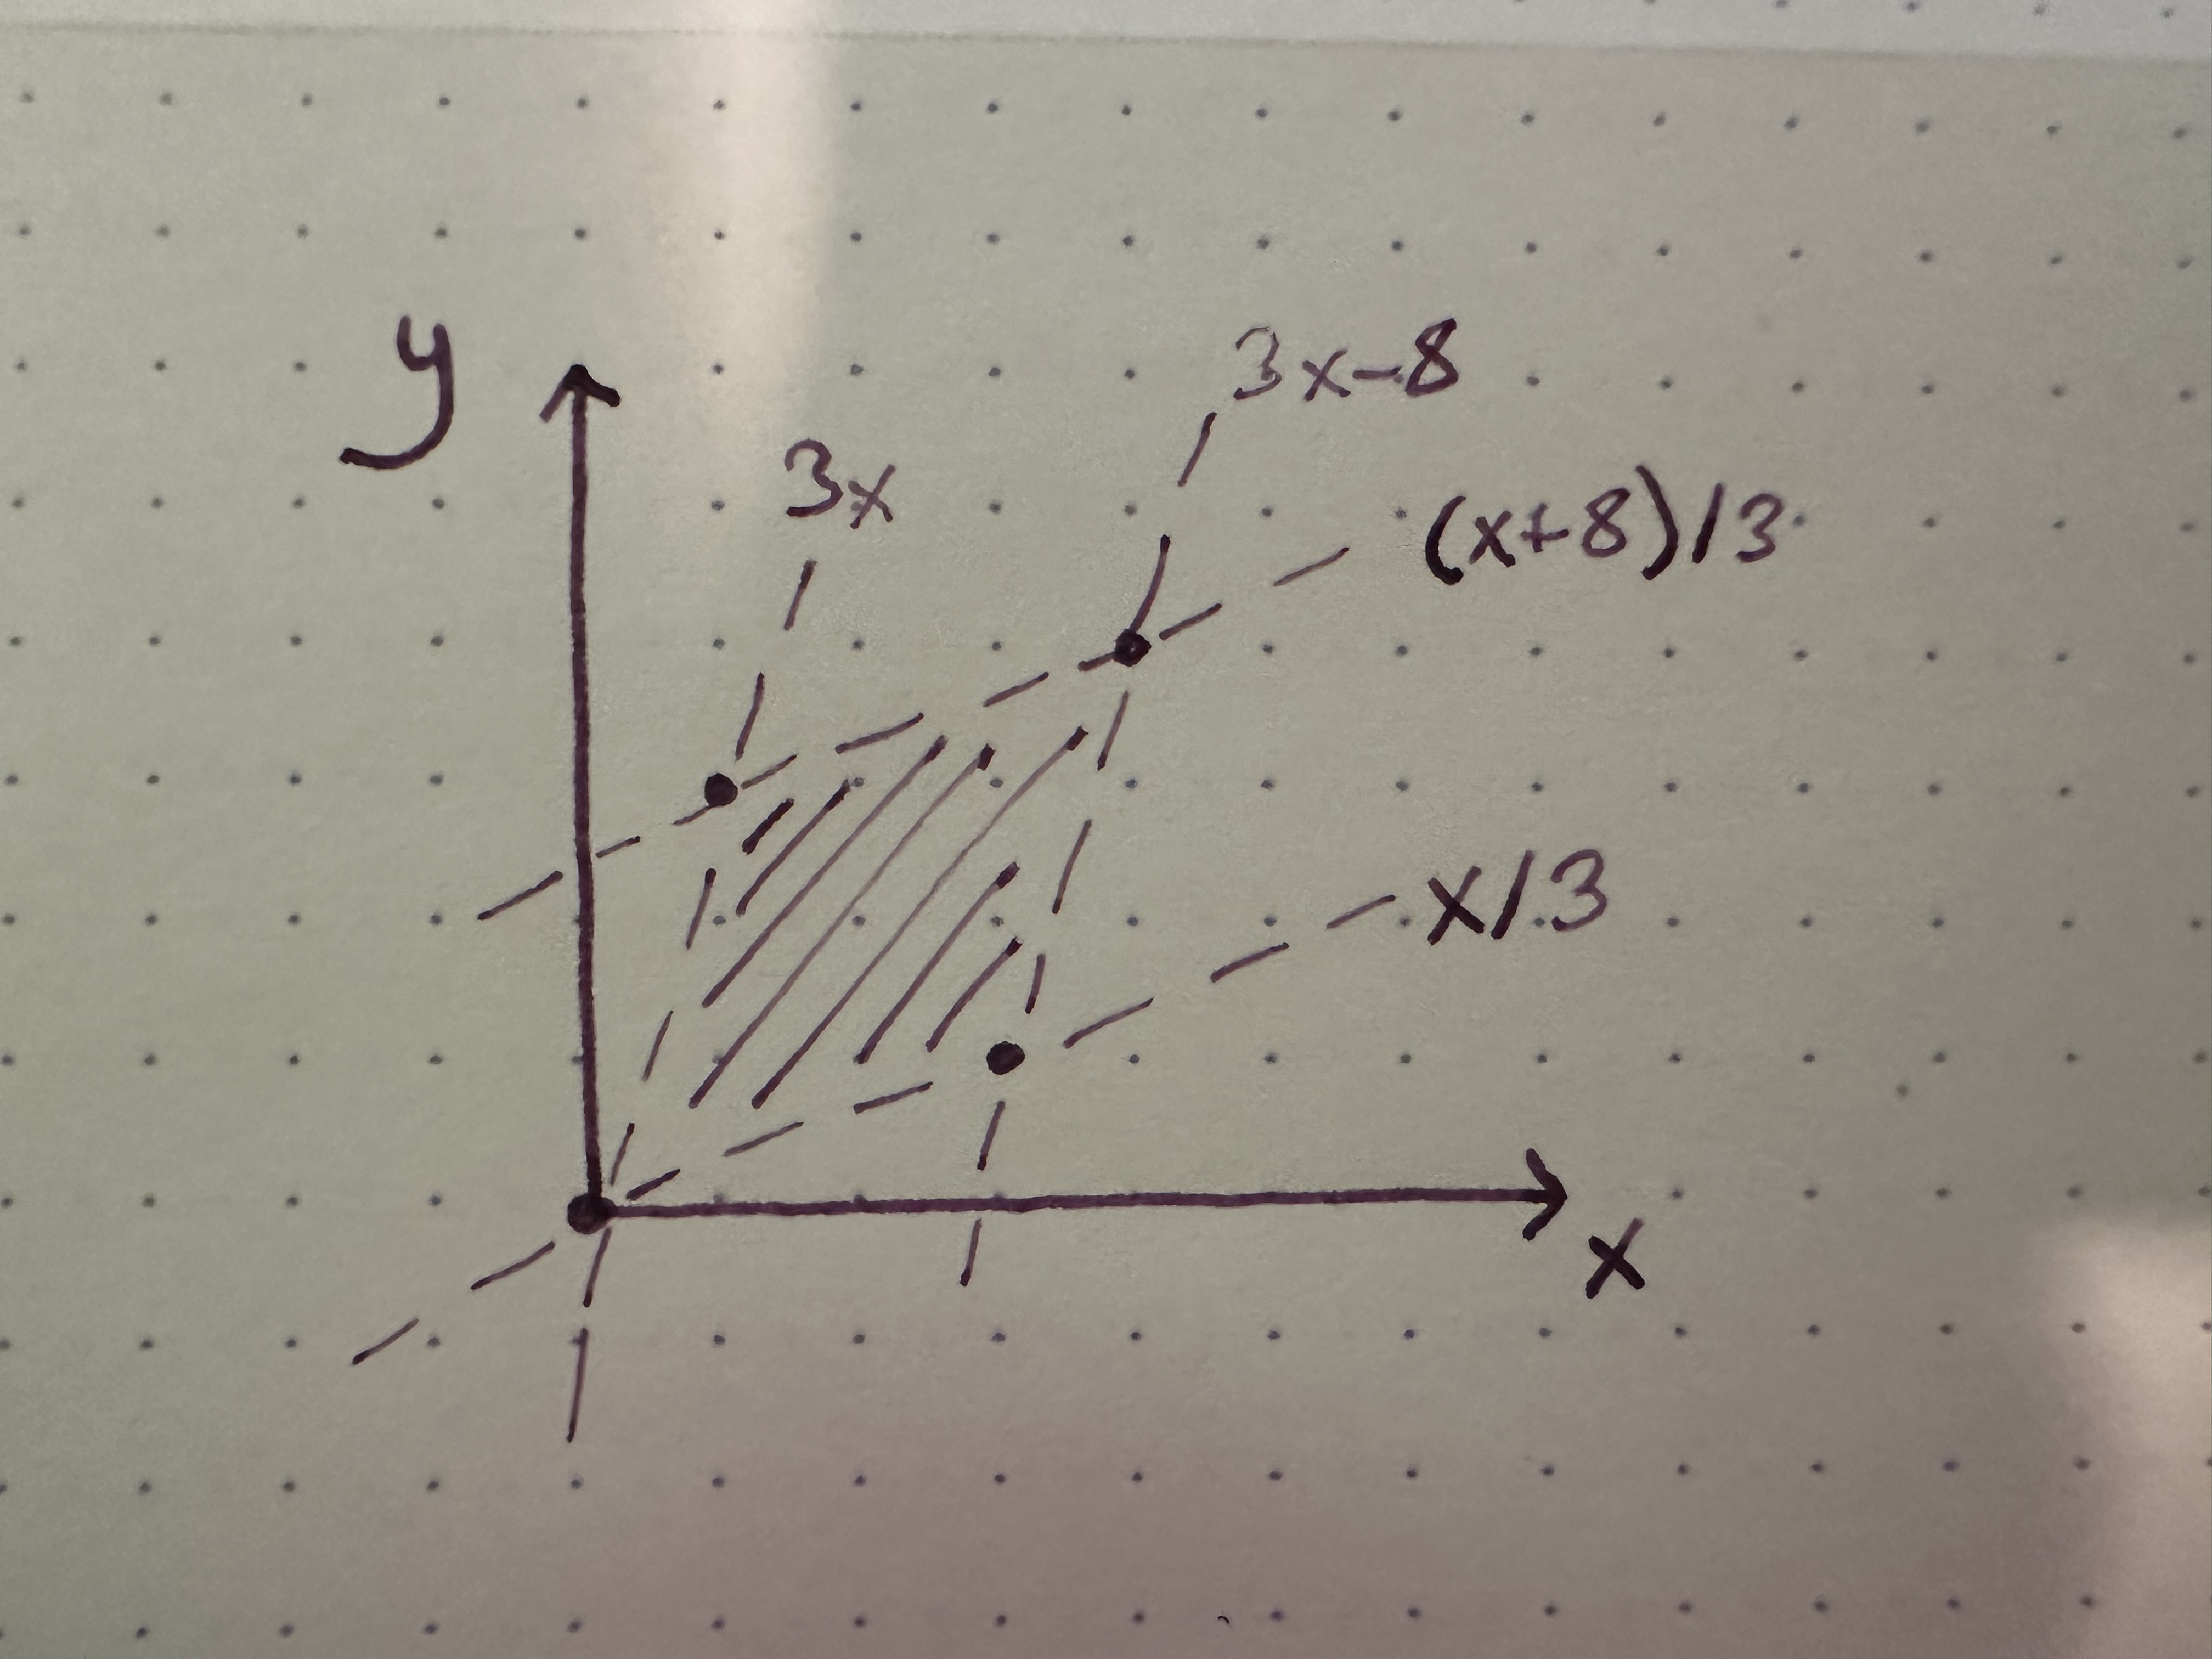
\includegraphics[height=40mm]{E2TH1.png}
  \label{fig:tree}
\end{figure}

\FloatBarrier

\subsection*{b)}

The integral that results from the pdf over its support is absolutely horrible. I'm going to change variables. Let $x=3u+v$ and $y=u+3v$ where the support is now $u\in [0,1]$, $v\in [0,1]$. The determinant of our Jacobian is:

$$
\det{\begin{bmatrix}
    \frac{\partial x}{\partial u} & \frac{\partial x}{\partial v} \\
    \frac{\partial y}{\partial u} & \frac{\partial y}{\partial v}
\end{bmatrix}}
=
\det{\begin{bmatrix}
    3 & 1 \\
    1 & 3
\end{bmatrix}}
= 9 - 1 = 8
$$

So 

$$f_{U,V}(u,v)=f_{X,Y}\left(x(u,v), y(u,v)\right)8$$

$$=8k(3u + v)^2(3v + u)=8k\left(9 u^3 + 33 u^2 v + 19 u v^2 + 3 v^3\right)$$

So now we want to evaluate the following:

$$\int_0^1 \int_0^1 8k\left(9 u^3 + 33 u^2 v + 19 u v^2 + 3 v^3\right)dvdu$$

$$=8k\int_0^1 \left(9u^3 + \frac{33}{2}u^2 + \frac{19}{3}u+\frac{3}{4}\right)du$$

$$=8k\left(\frac{9}{4} + \frac{33}{6} + \frac{19}{6}+\frac{3}{4} \right)=8k\frac{27+66+38 + 9}{12}=\frac{280k}{3}$$


Therefore $k=\frac{3}{280}$.




\subsection*{c)}

In this case $P(X+Y<1)=P(3U+V + 3V + U < 1)= P(U+V < 1/4)$. 

\begin{figure}[h!] 
	\centering
  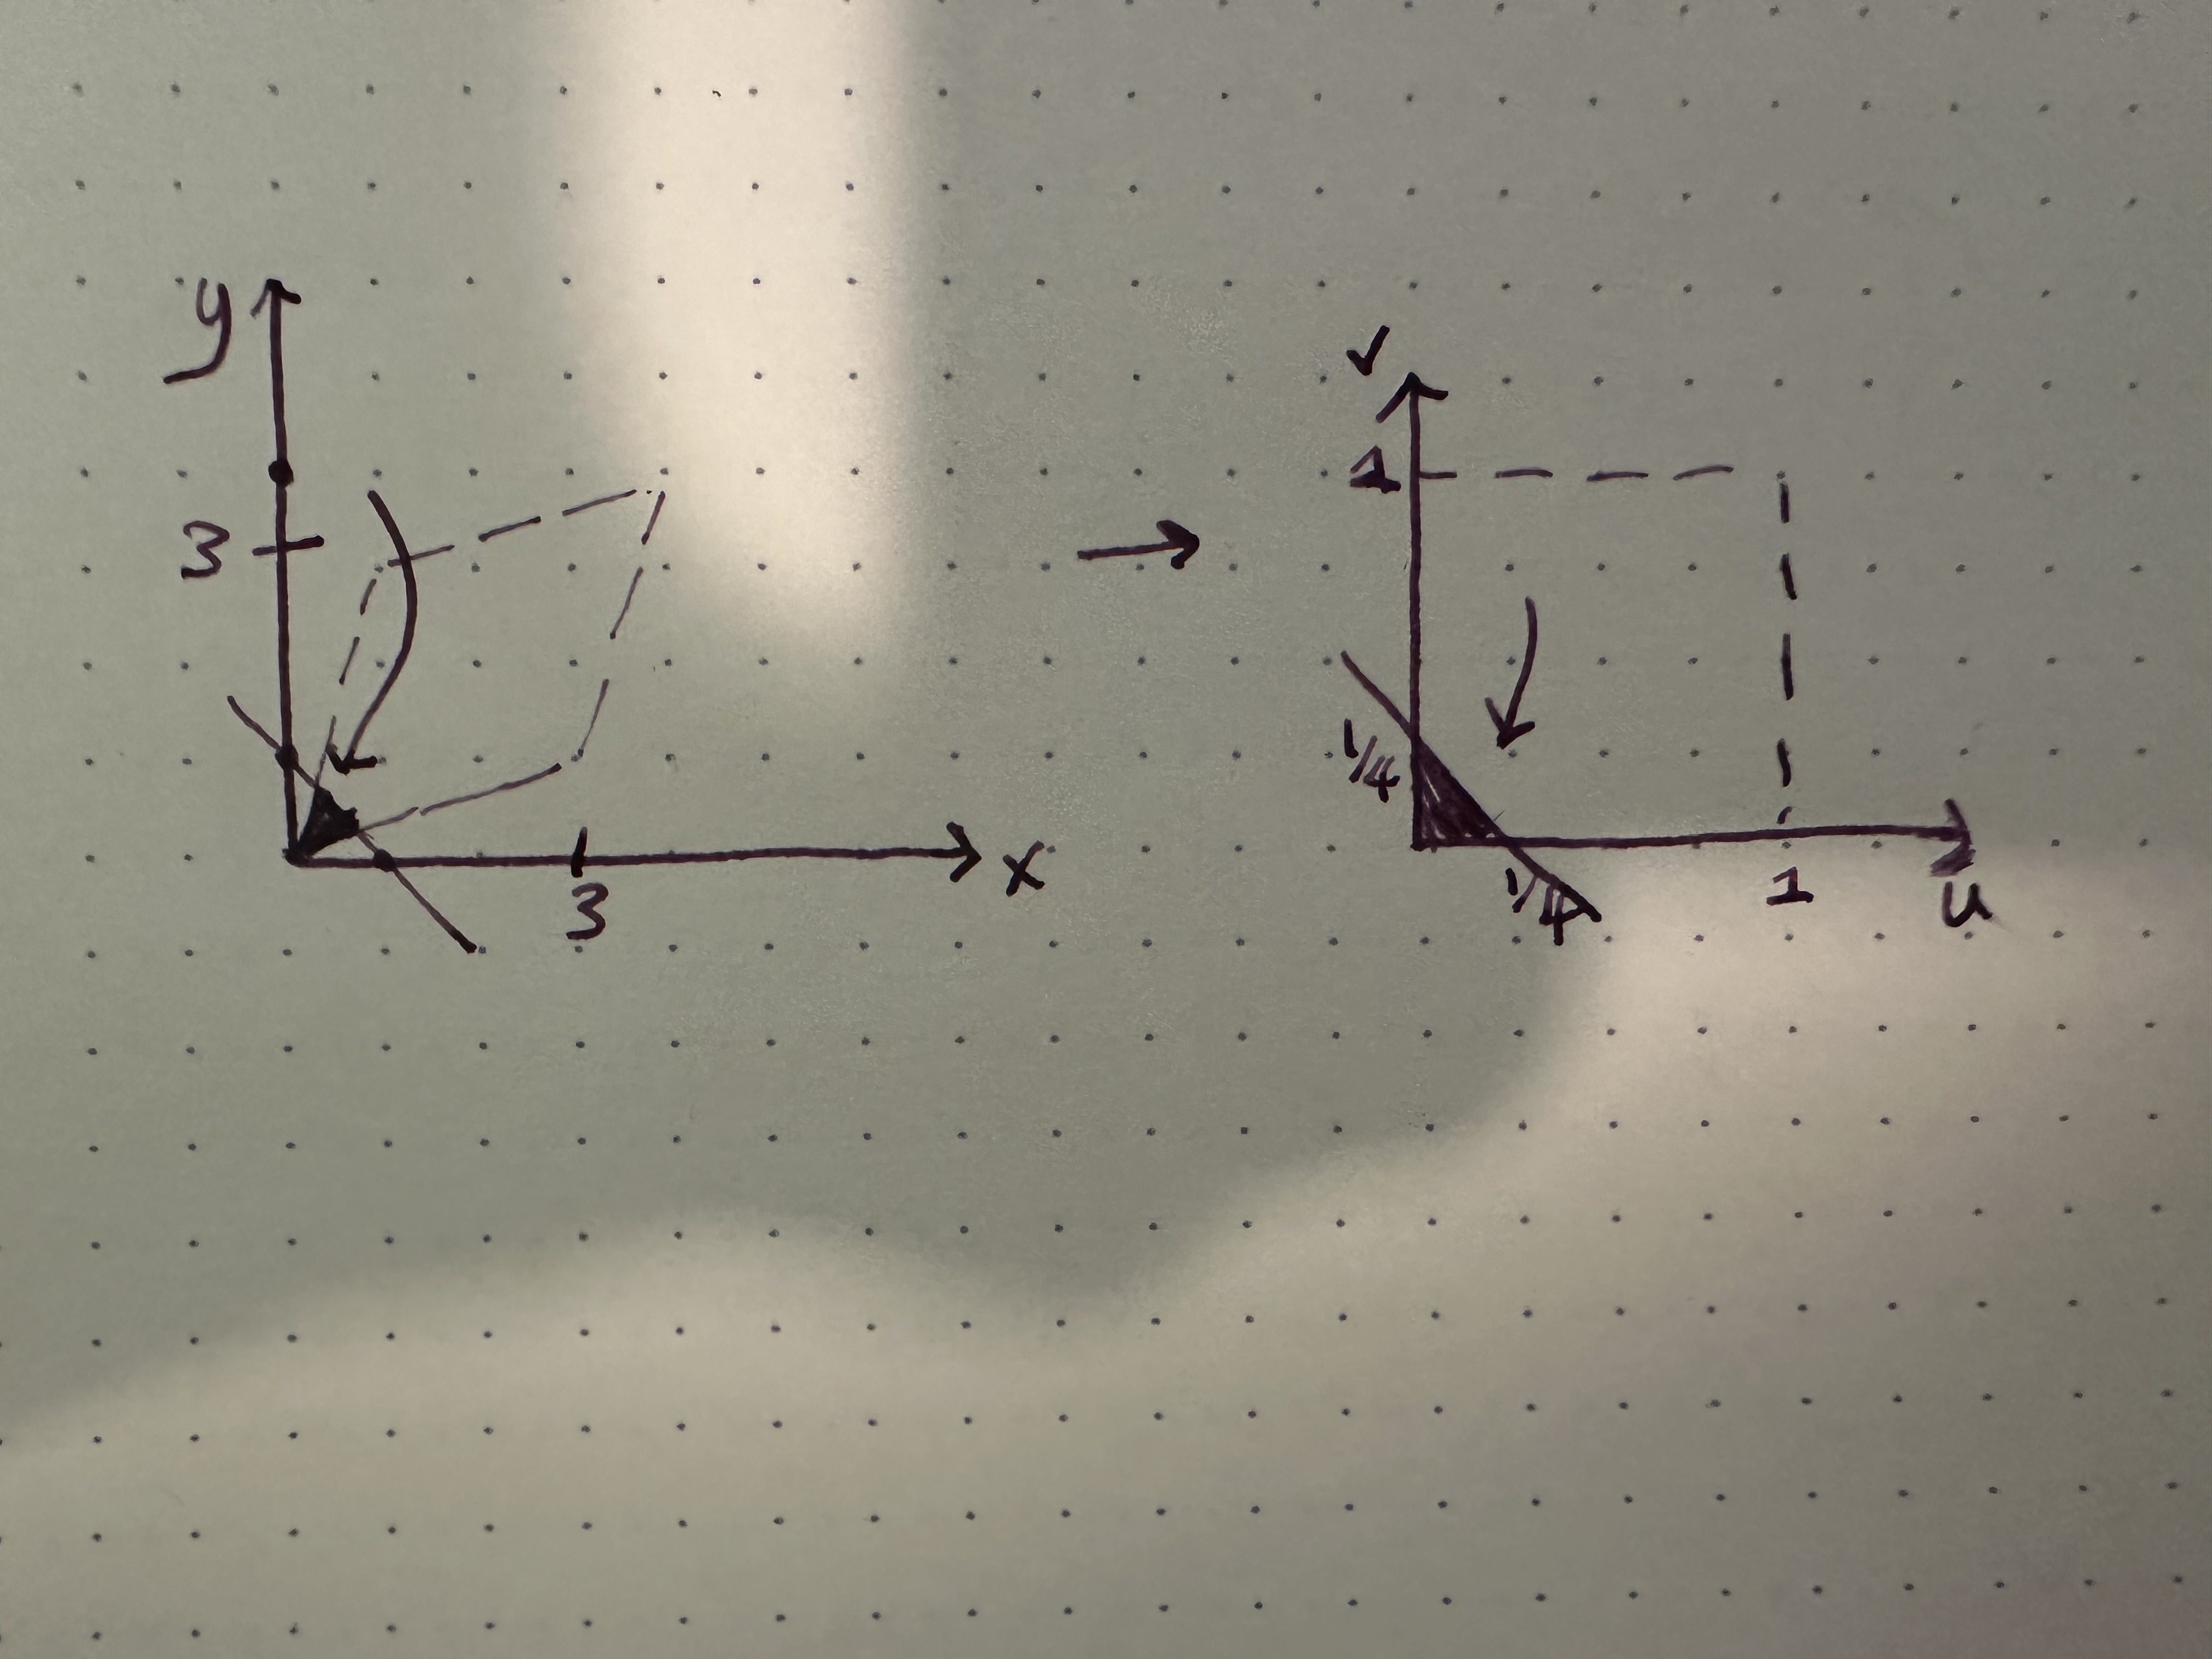
\includegraphics[height=40mm]{E2TH2.png}
  \label{fig:tree}
\end{figure}

\FloatBarrier

So we have:

$$\int_0^{1/4} \int_0^{1/4-u} 8k\left(9 u^3 + 33 u^2 v + 19 u v^2 + 3 v^3\right)dvdu$$
$$=\frac{11k}{960}=\frac{11}{89600}$$

\subsection*{d)}

$$P(Y>X) = P(3V+U > 3U + V) = P(V>U)$$

\begin{figure}[h!] 
	\centering
  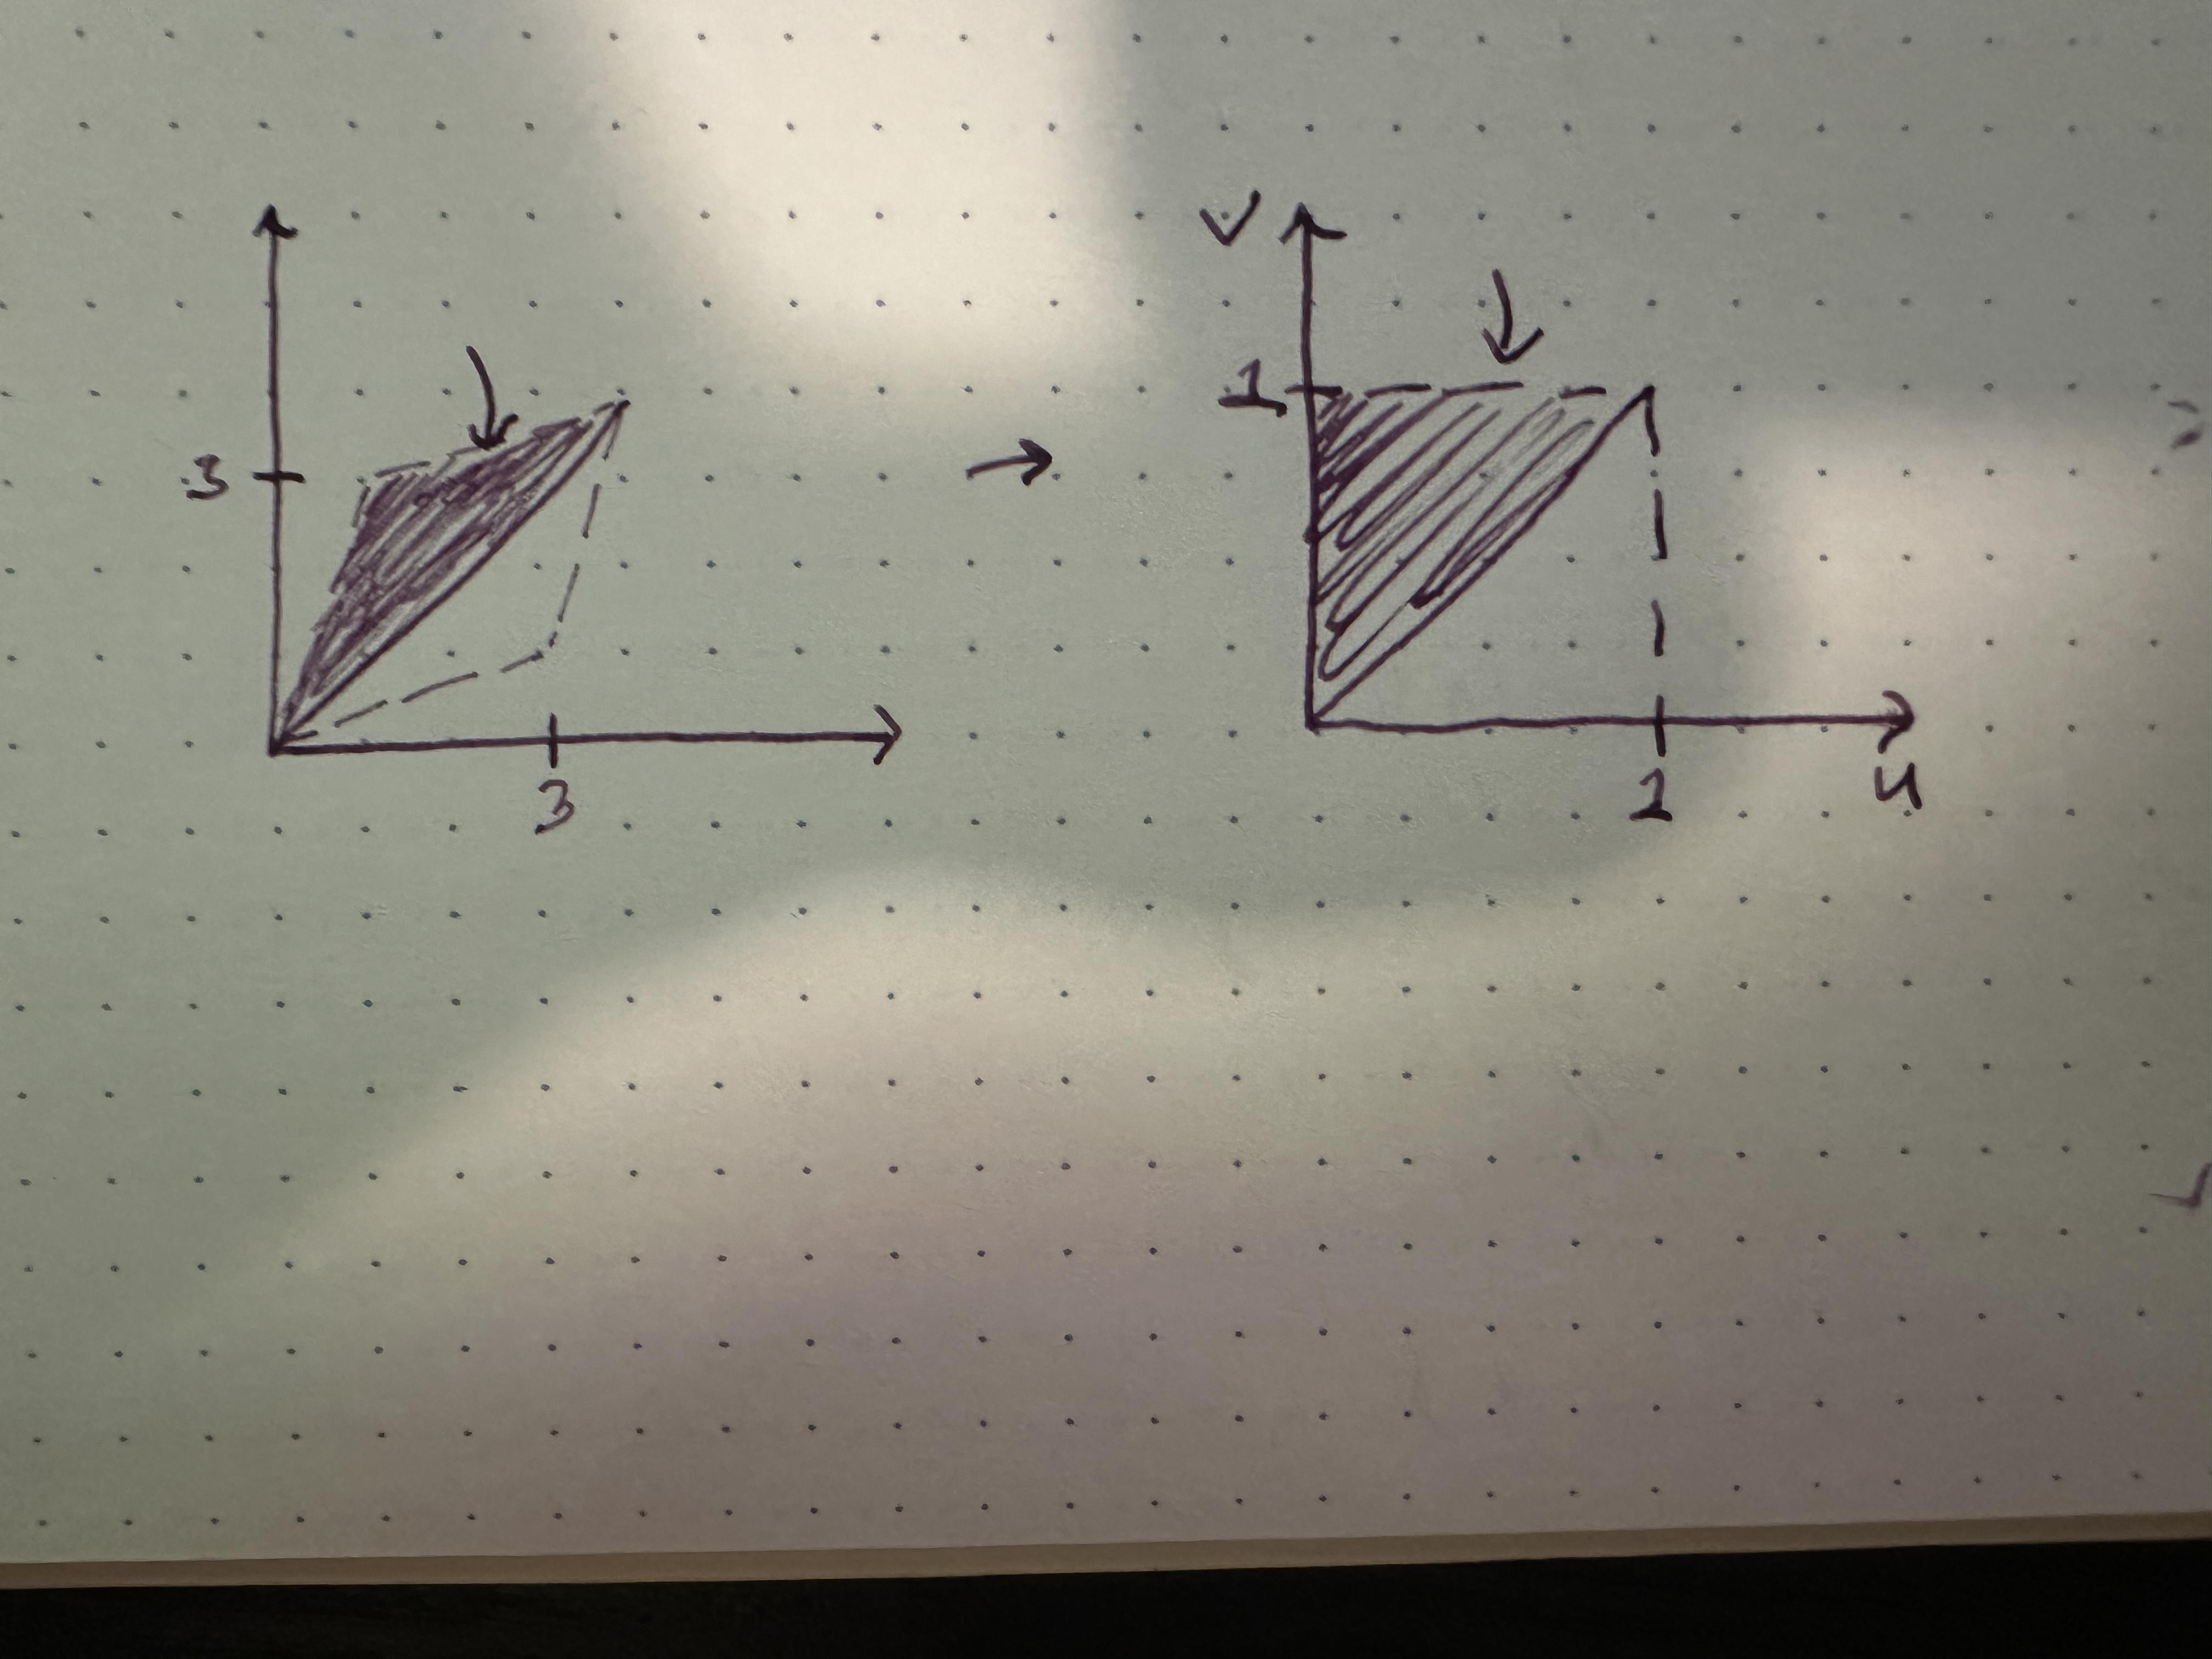
\includegraphics[height=40mm]{E2TH3.png}
  \label{fig:tree}
\end{figure}

\FloatBarrier

Therefore we're wanting to evaluate:

$$\int_0^{1} \int_u^{1} 8k\left(9 u^3 + 33 u^2 v + 19 u v^2 + 3 v^3\right)dvdu=\frac{206k}{5}=\frac{309}{700}$$

\subsection*{e)}

We have a few cases: \newline

\textbf{If $0\leq y < 1$:}

$$f_Y(y) = \int_{y/3}^{3y}kx^2ydx=\frac{728ky^4}{81}$$\newline

\textbf{If $1\leq y < 3$:}

$$f_Y(y) = \int_{y/3}^{(y+8)/3} kx^2ydx= \frac{8k}{81} y (3 y^2 + 24 y + 64)$$\newline

\textbf{If $3 \leq y\leq 4$:}

$$f_Y(y) = \int_{3y-8}^{(y+8)/3}kx^2ydx= \frac{k}{81} y ((y + 8)^3 - 27 (3 y - 8)^3)$$

In summary:

$$
f_Y(y) = \begin{cases}
    \frac{728ky^4}{81} & \text{if } 0\leq y < 1 \\
    \frac{8k}{81} y (3 y^2 + 24 y + 64) & \text{if } 1\leq y < 3 \\
    \frac{k}{81} y ((y + 8)^3 - 27 (3 y - 8)^3) & \text{if } 3 \leq y\leq 4
\end{cases}
$$

so is this a pdf? 

$$\int_0^1 \frac{728ky^4}{81}dy = \frac{728k}{405}$$

$$\int_1^3 \frac{8k}{81} y (3 y^2 + 24 y + 64)dy = \frac{4192k}{81}$$

$$\int_3^4 \frac{k}{81} y ((y + 8)^3 - 27 (3 y - 8)^3)dy = \frac{16112k}{405}$$

$$\frac{728k}{405}+\frac{4192k}{81}+\frac{16112k}{405}=\frac{280k}{3}=1$$

This is indeed a pdf. 

\newpage

\section*{Question 3}

\subsection*{a)}

\begin{figure}[h!] 
	\centering
  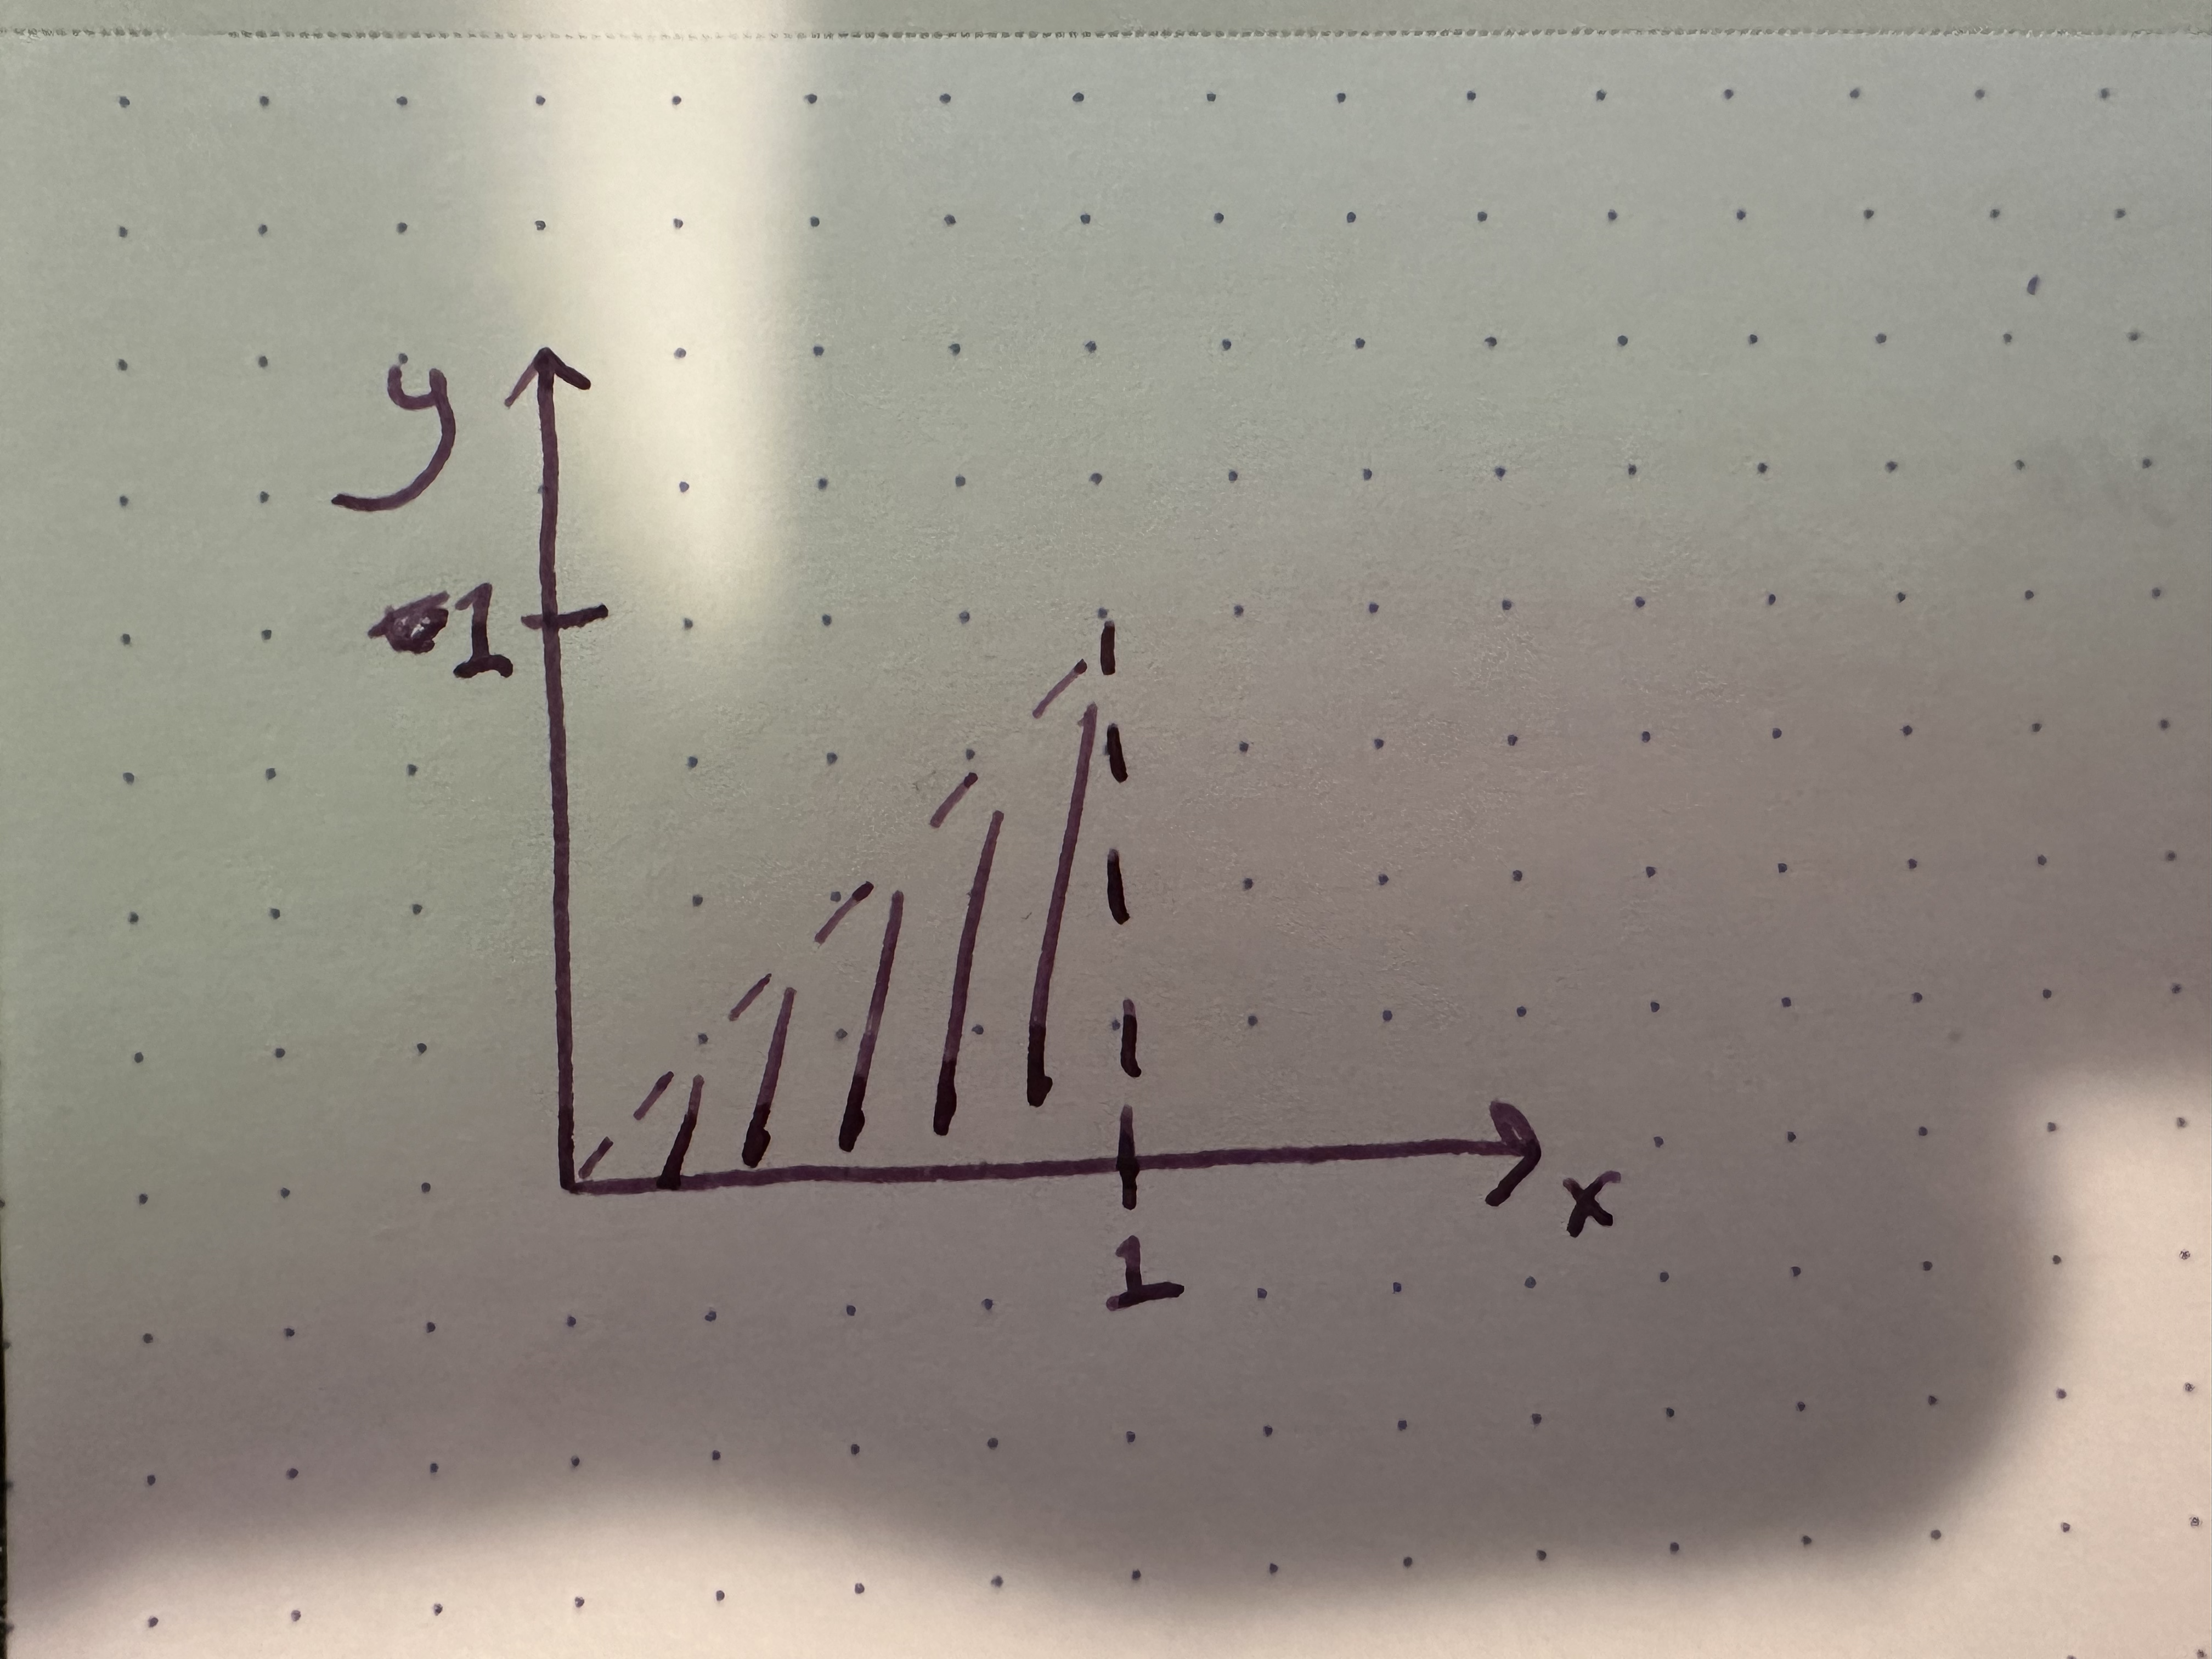
\includegraphics[height=40mm]{E2TH4.png}
  \label{fig:tree}
\end{figure}

\FloatBarrier


\subsection*{b)}

\begin{figure}[h!] 
	\centering
  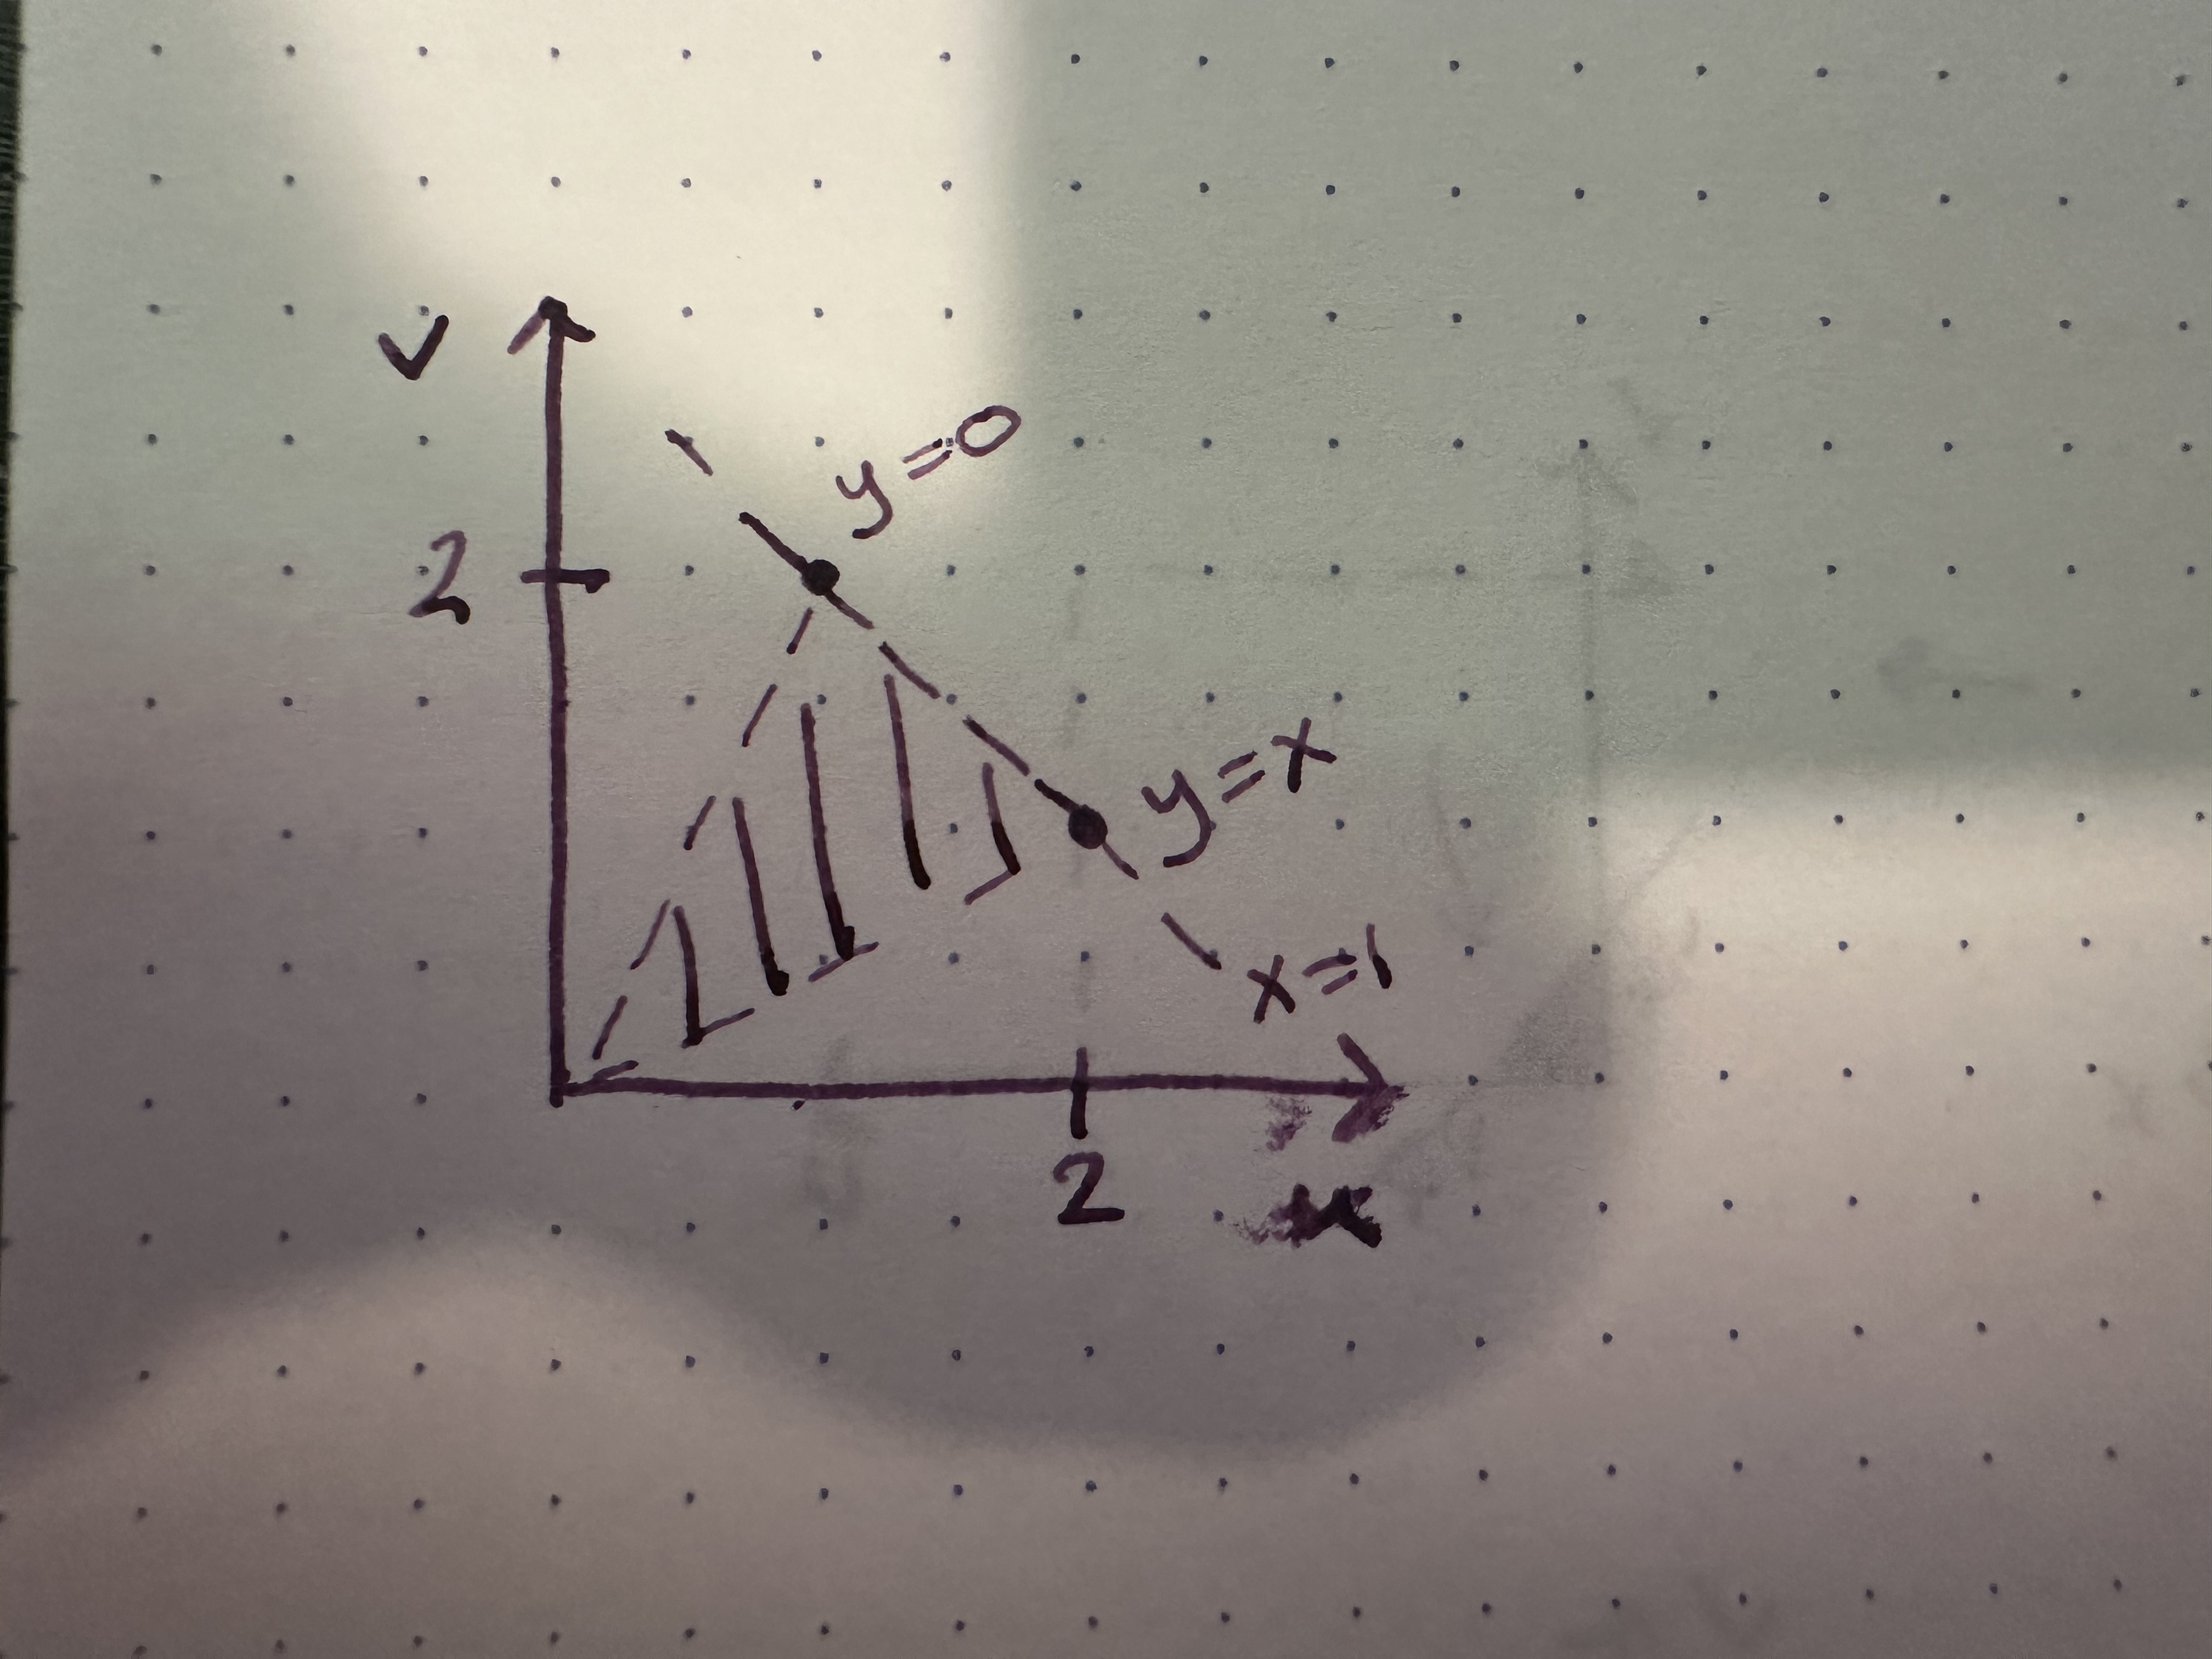
\includegraphics[height=40mm]{E2TH5.png}
  \label{fig:tree}
\end{figure}

\FloatBarrier

\subsection*{c)}

In this case we find that $x=(u+v)/3$ and $y=(2u-v)/3$. Therefore the determinant of our Jacobian is:

$$
\det{\begin{bmatrix}
    \frac{\partial x}{\partial u} & \frac{\partial x}{\partial v} \\
    \frac{\partial y}{\partial u} & \frac{\partial y}{\partial v}
\end{bmatrix}}
=
\det{\begin{bmatrix}
    1/3 & 1/3 \\
    2/3 & -1/3
\end{bmatrix}}
= -1/9 - 2/9 = -1/3
$$

and so we have:

$$f_{U,V}(u,v) = \frac{2}{3}uI(0\leq u \leq 2, u/2 \leq v \leq 2u, v\leq 3-u)$$

\subsection*{d)}

There is no way to factor the $I$ in the above given the support is not rectangular. Therefore $U$ and $V$ are not independent. 




\end{document}